% ============================================================
%  第三卷 第八章 自旋（§54–§60 + 习题）
%  底本：高教社中文版第6版（严肃译）；OCR 错误已修正
%
%  已修正的 OCR / 原书错误（对照原书页面 PNG p197–p221 逐条核实）：
%  1. §54：OCR 在"也可以是某些方面类似于基本粒子的一个复合粒子"句中误插
%     重复圈码②（原书 p185 仅"轨道角动量②"一处），已删；
%  2. §54：OCR 漏"下列积分"四字（自旋分量讨论前，p185），已补；
%  3. §54：轨道角动量记号 OCR 作"1"，按原书 p187 为粗体 \boldsymbol{l}；
%     "总角动量可取…|l−s| 等值"OCR 乱码"1l−s1"已恢复；
%  4. §54 习题解：w_± 下标丢失（OCR 作 w_.），按原书 p187 补为 w_+ − w_-；
%     两处 \tilde{s}_{z'} 按原书均为平均值 \bar{s}_{z'}；
%  5. §54：OCR"绕γ轴连接"按原书 p186 为"绕 y 轴连接"；"i算符"按 p186
%     为 \hat{l}_z 算符（(26.14) 式），"推 L_z 导"为"推导…L_z 分量"错位；
%  6. §55 (55.5) 第二行：OCR 作 −(s_x)_{σ−1,σ}，按原书 p189 为 −(s_y)_{σ−1,σ}；
%  7. §55 (55.8) 第二行第三式：OCR 作 σ̂_zσ̂_y=iσ̂_z，按原书 p189 为
%     σ̂_xσ̂_y=iσ̂_z；"矩阵 ŝ_z=½σ̂_z"OCR 漏 σ 的下标 z，按原书补；
%  8. §56：OCR"变换矩阵Φ"按原书 p191 为脚注圈码"变换矩阵①"；
%  9. §56 (56.13) 前：OCR"Ũ*=Ũ⁻¹"按原书 p193 为 Ũ*=Û⁻¹；
% 10. §56：高秩旋量定义处 OCR 作 ψ^μ，按原书 p193 为 ψ^{λμ}；
%     逆矩阵 (d,−b;−c,·) 漏元素 a，按原书补；
% 11. §57：旋量分量指标串的计数标记（s+σ、s−σ / j+m、j−m）OCR 全乱
%     （"45÷⋯1⋯2""20/4¹4¹⋯"等），按原书 p195–196 重建为
%     \overset/\underset 记号；(57.1) 第二求和限 λ,μ,⋯=1..2 补齐；
% 12. §57 (57.4)：OCR 夹杂乱码 \hat{\xi}、上标撇号，按原书 p196 改为指标 1,2；
% 13. §58 (58.4)：Û_x 矩阵 OCR 漏虚数单位，按原书 p200 为 i sin(φ/2)；
%     矩阵乘积式 OCR 作 Û_γ(β)，按原书 p201 为 Û_y(β)；
% 14. §58 (58.8)、(58.22) 两表 OCR 全乱，按原书 p201/p203 重建
%     （m 列标、m′ 行标，角部斜线以 \diagdown 近似）；
% 15. §58 (58.10)：雅可比多项式下标按原书 p202 为 j−m′（OCR 作 j−m）；
% 16. §58 (58.20)：末因子按原书 p203 为 δ_{m′₁m′₂}（OCR 作 δ_{m₁m′₂}）；
% 17. §59：OCR 将 (59.3) 式体与其说明文字错位、"ρ^{λμ} 条件"残句，
%     按原书 p204 重建为"电子的自旋密度矩阵或极化密度矩阵是一个二秩旋量
%     ρ^λ_μ，满足以下归一化条件：…(59.1)…(59.2)…(59.3)"；
% 18. §59：ψ^{λ+} 按原书 p205 为 ψ^{λ*}；(59.8) 上标按 p205 为复共轭 *；
% 19. §60：(60.1)(60.2) OCR 漏复共轭 *，按原书 p206 补；
%     ψ^{λμν}=ψ_{λμ} 按原书 p208 为 ψ^{λμ*}=ψ_{λμ}；"对应干"→"对应于"；
% 20. 其它：\mathrm{d} 收紧、函数名正体（\cos、\sin、\exp、tr）、
%     e^{ıσφ}→e^{iσφ}、ψ(x,y,z;σ) 的粗体变量收紧、
%     "对应干/连接"等文字按原书校正。
%
%  遗留问题（OCR 存疑，已照原书排版）：
%  - §57 (57.2)(57.5) 等处旋量分量指标串上的计数标记为排版重建，
%    与原书小字上标的位置或略有出入；
%  - (58.8)(58.22) 表角部 m/m′ 斜线分隔系近似原书样式；
%  - §54"连接进行两次无限小旋转"照原书 p186 排（语义似应为"接连"）；
%  - (58.4) 末尾标点 OCR 作逗号，按文意排句点。
%
%  脚注（脚注代理，2026-10-11，按原书页面 p197–p221 逐页核录，共 29 处）：
%  - 圈码 29 处全部还原为 \footnote；对照表缺漏 9 处按 content_list 页索引+页面
%    实况定位：§55"任意矢量③"→ p202；§56"变换矩阵①"→ p204、"(ψÛ⁻¹)_λ 或①"
%    → p206；§57"独立分量数②"→ p211；§58 欧拉角①→ p213、D^{(1/2)}①→ p214、
%    d 函数①→ p215、雅可比多项式②→ p215；§60"双重简并①"→ p221；
%  - 页界偏差：对照表 p218 的"独立分量数①"实际在 p219（该页兼含 §60 开头，
%    "下列变换②"亦在 p219），p220 的"双重简并①②"实际在 p221（以页面脚注区为准）；
%  - 公式类脚注：§55②（ψ_σ1(σ)=ψδ_σ1σ）、§55①（泡利矩阵行乘列矩阵式）、
%    §57①（ψ=Σa_mψ_jm 三式）、§58①（欧拉角关系 φ=α+½π 等）、§58①（(58.7)
%    行乘列式）均按原书完整转录；
%  - §58 雅可比多项式脚注引 A. R. Edmonds, Angular Momentum in Quantum
%    Mechanics, Princeton, 1957（原书两处均作 Edmonds）。
% ============================================================
\chapter{自旋}

\section{自旋}

经典力学和量子力学中，角动量守恒定律都是封闭系统空间各向同性的结果，这一点，早已用角动量和旋转对称性之间的关系论述过.但在量子力学中，这个关系具有特别深远的意义，它确定了角动量这个概念的基本内容，特别是由于粒子角动量的经典定义 $\boldsymbol{r}\times\boldsymbol{p}$ 在量子力学中不再具有直接含义，因为位置和动量不能同时测量.

我们在§28中看到，如果 $l$ 和 $m$ 的值已给定，粒子波函数的角部关系就被确定，从而它在旋转下的所有对称性质也被确定.这些性质最一般的表述可归结为波函数在坐标系转动下的变换规律.

多粒子系统的波函数 $\boldsymbol{\Psi}_{LM}$（角动量 $L$ 及其分量 $M$ 的值业已给定）只有当坐标系绕 $z$ 轴转动时才能保持不变\footnote{除了一个不重要的相位因子外.}，任何改变 $z$ 轴方向的转动，结果都会使角动量 $z$ 分量没有定值.这意味着，在新的坐标系中，这个波函数一般变为具有给定 $L$ 值但有不同 $M$ 值的 $2L+1$ 个函数的叠加（即线性组合）.我们可以说，坐标系转动后，$2L+1$ 个函数 $\boldsymbol{\Psi}_{LM}$ 变成了它们相互的线性组合\footnote{用数学术语来说，这组函数构成了旋转群的一个不可约表示.得以进行相互线性变换的这组函数中的独立函数的个数，称为该表示的维数；并且这个数在函数组的相互线性变换中不可能再少.}.其变换规律（即组合系数与坐标轴转动角之间的函数关系）完全由 $L$ 值确定.因此角动量被赋予量子数的含义，它能对一个系统的各个态按照坐标系转动下的变换性质加以分类.角动量概念的这一方面，在量子力学中特别重要，因为它和角部波函数的显示式没有直接的联系；不用这些显示式也能表出这组函数的相互变换规律.

我们来考虑一个复合粒子，例如一个原子核，它整个地静止并且处于某一确定内部状态中.除了内能外，由于核内粒子的运动，它还具有确定的角动量值 $L$.这个角动量可以有 $2L+1$ 种不同的空间取向.因此，当我们考虑这个复合粒子的整体运动时，除了坐标外，还必须增加一个离散变量：它的内部角动量在空间某一选定方向上的投影.

根据我们对角动量概念的上述理解，有关它的起源问题显得并不重要.我们可以从中归结出“内禀”角动量的概念，用以描述粒子，不管这个粒子是“复合”的还是“基本”的.

因此，在量子力学中，每个基本粒子必须赋予一个与其空间运动无关的“内禀”角动量.基本粒子的这个性质是量子理论中特有的（在 $\hbar\to0$ 的极限下消失），因此在原则上不存在经典解释\footnote{例如，把基本粒子的内禀角动量想象为“绕自身轴”旋转的结果，这是完全没有意义的.}.

一个粒子的内禀角动量称为该粒子的自旋，以便区别于粒子空间运动所产生的角动量，所谓轨道角动量\footnote{电子具有内禀角动量的物理概念是由 G.~乌伦贝克（Uhlenbeck）和 S.~高兹米特（Goudsmit）于 1925 年提出的. 1927 年 W.~泡利（Pauli）把自旋引入量子力学中.}.我们所讲的粒子可以是一个基本粒子，也可以是某些方面类似于基本粒子的一个复合粒子（例如一个原子核）.一个粒子的自旋（和轨道角动量一样，以 $\hbar$ 为量度单位）用 $s$ 来代表.

对于有自旋的粒子，用波函数描述其状态时，这个波函数必须不但能确定该粒子处于不同空间位置的概率，而且也能确定其自旋具有各种可能取向的概率.因此，这个波函数不但依赖于三个连续变量，即粒子的三个坐标，而且还依赖于一个离散的自旋变量，它给出自旋在空间某一指定方向（$z$ 轴）的投影并取为数有限的离散值，我们用 $\sigma$ 代表这个自旋变量.

令 $\psi(x,y,z;\sigma)$ 为这样的波函数.实质上它代表了对应于不同 $\sigma$ 值的一组不同的坐标函数；这些函数称为波函数的各个自旋分量.下列积分
\begin{equation*}
  \int|\psi(x,y,z;\sigma)|^2\,\mathrm{d}V
\end{equation*}
确定了粒子具有某个 $\sigma$ 值的概率.粒子具有任意的 $\sigma$ 值并处于 $\mathrm{d}V$ 体积元内的概率为
\begin{equation*}
  \mathrm{d}V\sum_{\sigma}|\psi(x,y,z;\sigma)|^2.
\end{equation*}

量子力学的自旋算符，作用于波函数的自旋变量 $\sigma$ 上.换句话说，它以某种方式把波函数的各个分量进行相互线性变换.这个算符的形状将在以后建立.但从最一般的考虑很易知道，算符 $\hat{s}_x,\hat{s}_y,\hat{s}_z$ 应该满足和轨道角动量一样的对易关系.

角动量算符和无限小旋转算符基本上相同.在§26中推导轨道角动量算符的具体表式时，我们考虑了旋转算符作用在一个坐标函数上所得的结果.在自旋的情形下，这一推导失去意义，因为自旋算符不是作用在坐标上，而是作用在自旋变量上的.因此，为了求得对易关系式，我们必须把一般形式的无限小旋转操作看作一般的坐标系旋转.如果我们先绕 $x$ 轴再绕 $y$ 轴连接进行两次无限小旋转，或者把次序倒过来，先绕 $y$ 轴再绕 $x$ 轴，经过直接计算后很易证明，以上两种操作结果的差别等于绕 $z$ 轴的一个无限小旋转（转过的角度等于绕 $x$ 轴和 $y$ 轴的两个转角的乘积）.我们不准备进行这种简单的计算，它的结果仍得通常的角动量分量算符之间的对易关系式；由此可见，这一对易关系式对自旋算符讲来也必成立：
\begin{equation}
  [\hat{s}_y,\hat{s}_z]=i\hat{s}_x,\quad
  [\hat{s}_z,\hat{s}_x]=i\hat{s}_y,\quad
  [\hat{s}_x,\hat{s}_y]=i\hat{s}_z.
\end{equation}
由这个关系式导出的所有物理结论也都应成立.

对易关系式(54.1)能使我们求出所有可能的自旋绝对值和所有可能的自旋分量值.§27中导出的所有结果［(27.7)—(27.9)式］仅仅应用了对易关系式，因此这些结果在这里也能全部适用，只要把上述各式中的 $\boldsymbol{L}$ 换成 $s$ 就可以了.根据(27.7)式，自旋 $z$ 分量的本征值是递差数为 1 的一组数值.但是我们不能像轨道角动量的 $\boldsymbol{L}_z$ 分量那样断定这些数值一定都是整数［§27之初给出的推导在这里不能成立，因为它是以(26.14)式的 $\hat{l}_z$ 算符为基础的，这个表式只对轨道角动量成立］.

其次，$s_z$ 这套本征值具有上下限，这两个上下限的绝对值相等而符号相反，我们用 $\pm s$ 表示之.$s_z$ 的最大值和最小值之差 $2s$ 必须是一个整数或零.因此 $s$ 可取 $0,\frac{1}{2},1,\frac{3}{2},\cdots$ 值.

于是，自旋平方的本征值等于
\begin{equation}
  s^2=s(s+1),
\end{equation}
其中的 $s$ 可以是一个整数（包括零）也可以是一个半整数.$s$ 给定后，自旋的 $s_z$ 分量可取 $s,s-1,\cdots,-s$ 等 $2s+1$ 个不同的数值.因此，自旋为 $s$ 的粒子波函数具有 $2s+1$ 个分量\footnote{由于每类粒子的 $s$ 是一个给定值，故在经典力学极限情形下（$\hbar\to0$）自旋角动量 $\hbar s$ 趋于零.对轨道角动量讲来由于 $l$ 可取任意值，这样的论证就失去意义.过渡到经典力学时，$\hbar$ 趋于零同时 $l$ 趋向无穷大，可是乘积 $\hbar l$ 仍为有限值.}.

实验表明，大多数的基本粒子［电子，正电子，质子，中子，$\mu$ 子和所有的超子 $(\Lambda,\Sigma,\Xi)$］具有 $\frac{1}{2}$ 的自旋.此外，也有些基本粒子（$\pi$ 介子和 K 介子）的自旋等于零.

一个粒子的总角动量等于它的轨道角动量 $\boldsymbol{l}$ 加上自旋 $\boldsymbol{s}$.这两个算符作用于函数的不同变量上，当然是彼此对易的.总角动量
\begin{equation}
  \boldsymbol{j}=\boldsymbol{l}+\boldsymbol{s}
\end{equation}
的本征值，与两个不同粒子的轨道角动量之和一样，取决于“矢量模型”的相加法则（§31）.这就是说，给定了 $l$ 和 $s$ 以后，总角动量可取 $l+s,l+s-1,\cdots,|l-s|$ 等值.因此，轨道角动量 $l$ 不等于零的一个电子（自旋为 $\frac{1}{2}$）具有总角动量 $j=l\pm\frac{1}{2}$；$l=0$ 时，$j$ 只有一个值 $j=\frac{1}{2}$.

多粒子系统的总角动量算符 $\hat{\boldsymbol{J}}$ 等于每个粒子的角动量算符 $\hat{\boldsymbol{j}}$ 之和，它的本征值仍用矢量模型法则加以确定.角动量 $\boldsymbol{J}$ 可以表成下列形状：
\begin{equation}
  \boldsymbol{J}=\boldsymbol{L}+\boldsymbol{S},\quad
  \boldsymbol{L}=\sum_a\boldsymbol{l}_a,\quad
  \boldsymbol{S}=\sum_a\boldsymbol{s}_a,
\end{equation}
其中的 $\boldsymbol{S}$ 可称为该系统的总自旋，$\boldsymbol{L}$ 可称为该系统的总轨道角动量.我们注意到，如果该系统的总自旋为半整数（整数），则总角动量也是半整数（整数），因为轨道角动量永远是整数.特别是，如果该系统是由偶数个同类粒子组成的，它的总自旋永远是整数，从而它的总角动量也是整数.

一个粒子的总角动量算符 $\hat{\boldsymbol{j}}$（或一个多粒子系统的 $\hat{\boldsymbol{J}}$），和轨道角动量算符或自旋算符满足同样的对易关系，这个关系是任意角动量所应满足的普遍的对易关系.由这个对易关系所导出的角动量矩阵元公式(27.13)，对任意的角动量讲来也都成立，只要这些矩阵元是由该角动量的本征态所定义的.对任意矢量的矩阵元，公式(29.7$\sim$10)也同样成立（改变相应的记号）.

\begin{xiti}

\noindent{\heiti 习题}\quad 自旋为 $\frac{1}{2}$ 的粒子处于 $s_z=\frac{1}{2}$ 的态中，求该自旋在 $z'$ 轴上的投影取各可能值的概率，设 $z'$ 轴和 $z$ 轴的夹角为 $\theta$.

解：平均后的自旋矢量 $\boldsymbol{s}$ 显然沿 $z$ 轴，且其数值等于 $\frac{1}{2}$.把它投影到 $z'$ 轴上，求得自旋沿 $z'$ 轴的平均值为 $\bar{s}_{z'}=\frac{1}{2}\cos\theta$.另一方面，我们又有 $\bar{s}_{z'}=\frac{1}{2}(w_+-w_-)$，其中的 $w_\pm$ 为 $s_{z'}=\pm\frac{1}{2}$ 的概率.考虑到 $w_++w_-=1$，我们得
\begin{equation*}
  w_+=\cos^2(\theta/2),\qquad w_-=\sin^2(\theta/2).
\end{equation*}

\end{xiti}

\section{自旋算符}

在本章以后各节中，我们不想讨论波函数与坐标的关系.例如，当我们讲到坐标系旋转后函数 $\psi(\sigma)$ 的行为时，我们可以假定该粒子处于原点，使得它的坐标在旋转中保持不变，这样得到的结果将标志出 $\psi(\sigma)$ 函数对自旋变量 $\sigma$ 而言的行为.

变量 $\sigma$ 和普通变量（坐标变量）的区别在于它的离散性.一个线性算符作用在离散变量 $\sigma$ 的函数上，所得的最普遍形式为
\begin{equation}
  (\hat{f}\psi)(\sigma)=\sum_{\sigma'}f_{\sigma\sigma'}\psi(\sigma'),
\end{equation}
其中的 $f_{\sigma\sigma'}$ 是一些常数.我们把 $\hat{f}\psi$ 放在括号内是为了强调在它后面所跟的自旋宗量不是属于原函数 $\psi$，而是属于用算符 $\hat{f}$ 作用后所得的那个函数.容易证明，$f_{\sigma\sigma'}$ 是和按通常规则(11.5)所定义的算符矩阵元一致的\footnote{注意(55.1)式右边矩阵元的下标次序与(11.11)式中的通常次序相反.}.

(11.5)中对坐标的积分现在换成对离散变量求和，所以矩阵元的定义为
\begin{equation}
  f_{\sigma_2\sigma_1}=\sum_{\sigma}\psi^*_{\sigma_2}(\sigma)[\hat{f}\psi_{\sigma_1}(\sigma)].
\end{equation}
其中 $\psi_{\sigma_1}(\sigma)$ 和 $\psi_{\sigma_2}(\sigma)$ 是算符 $\hat{s}_z$ 的本征函数，属于本征值 $s_z=\sigma_1$ 和 $\sigma_2$；每个函数对应于一个态，粒子处于此态时具有确定的 $s_z$ 值，亦即此时波函数只有一个分量不等于零\footnote{更明确地说，我们应写成
\begin{equation*}
  \psi_{\sigma_1}(\sigma)=\psi(x,y,z)\,\delta_{\sigma_1\sigma}.
\end{equation*}
(55.3)中略去了坐标因子，在那里并不重要.
我们必须再一次强调 $s_z$ 的特定本征值 $\sigma_1$ 或 $\sigma_2$ 有别于独立变量 $\sigma$.}：
\begin{equation}
  \psi_{\sigma_1}(\sigma)=\delta_{\sigma\sigma_1},\qquad
  \psi_{\sigma_2}(\sigma)=\delta_{\sigma\sigma_2},
\end{equation}
根据(55.1)，
\begin{equation*}
  (\hat{f}\psi_{\sigma_1})(\sigma)=\sum_{\sigma'}f_{\sigma\sigma'}\psi_{\sigma_1}(\sigma')
  =\sum_{\sigma'}f_{\sigma\sigma'}\delta_{\sigma'\sigma_1}=f_{\sigma\sigma_1}.
\end{equation*}
把上式及 $\psi_{\sigma_2}(\sigma)$ 的表式代入(55.2)，该式恒得到满足；证毕.

由此可见，作用于 $\sigma$ 的函数上的算符可以表成一个 $(2s+1)$ 行 $(2s+1)$ 列的矩阵.特别是自旋算符本身，作用在波函数上后，按(55.1)有
\begin{equation}
  (\hat{s}\psi)(\sigma)=\sum_{\sigma'}s_{\sigma\sigma'}\psi(\sigma').
\end{equation}
按照§54末段所述，矩阵 $\hat{s}_x,\hat{s}_y,\hat{s}_z$ 与§27所得的矩阵 $\hat{\boldsymbol{L}}_x,\hat{\boldsymbol{L}}_y,\hat{\boldsymbol{L}}_z$ 相同，只是把字母 $L$ 和 $M$ 改成 $s$ 和 $\sigma$：
\begin{equation}
\left.\begin{aligned}
  (s_x)_{\sigma,\sigma-1}&=(s_x)_{\sigma-1,\sigma}
  =\frac{1}{2}\sqrt{(s+\sigma)(s-\sigma+1)},\\
  (s_y)_{\sigma,\sigma-1}&=-(s_y)_{\sigma-1,\sigma}
  =-\frac{1}{2}i\,\sqrt{(s+\sigma)(s-\sigma+1)},\\
  (s_z)_{\sigma,\sigma}&=\sigma.
\end{aligned}\right\}
\end{equation}
这就确定了自旋算符.

在自旋为 $\frac{1}{2}$（$s=\frac{1}{2}$，$\sigma=\pm\frac{1}{2}$）的重要情形下，这些矩阵是两行两列的，具有下列形式
\begin{equation}
  \hat{\boldsymbol{s}}=\frac{1}{2}\hat{\boldsymbol{\sigma}},
\end{equation}
其中\footnote{(55.7)中所列的矩阵，行和列都按 $\sigma$ 的值编号，行数对应于矩阵元的第一个脚标，列数则对应于第二个脚标.目前情形下，这些编号数为 $\dfrac{1}{2}$ 和 $-\dfrac{1}{2}$.(55.4)式所示的算符，其作用是把矩阵的第 $\sigma$ 行乘以由波函数各个分量组成的一个列矩阵：
\begin{equation*}
  \psi=\left(\begin{array}{c}
  \psi\left(\dfrac{1}{2}\right)\\[1.2em]
  \psi\left(-\dfrac{1}{2}\right)
  \end{array}\right).
\end{equation*}}
\begin{equation}
  \hat{\sigma}_x=\left(\begin{array}{cc}0&1\\1&0\end{array}\right),\quad
  \hat{\sigma}_y=\left(\begin{array}{cc}0&-i\\i&0\end{array}\right),\quad
  \hat{\sigma}_z=\left(\begin{array}{cc}1&0\\0&-1\end{array}\right).
\end{equation}
这些矩阵称为泡利矩阵.矩阵 $\hat{s}_z=\frac{1}{2}\hat{\sigma}_z$ 确是对角的，因为它是用 $s_z$ 本身的本征函数组来定义的\footnote{用同一字母代表自旋分量和泡利矩阵，不会发生混淆.因为后者总是带有“\textasciicircum{}”符号.}.

下面是泡利矩阵的一些特殊性质.把(55.7)中的矩阵直接相乘，得下列方程：
\begin{equation}
\left.\begin{aligned}
  \hat{\sigma}_x^2&=\hat{\sigma}_y^2=\hat{\sigma}_z^2=1,\\
  \hat{\sigma}_y\hat{\sigma}_z&=i\hat{\sigma}_x,\quad
  \hat{\sigma}_z\hat{\sigma}_x=i\hat{\sigma}_y,\quad
  \hat{\sigma}_x\hat{\sigma}_y=i\hat{\sigma}_z.
\end{aligned}\right\}
\end{equation}
由上式及一般对易关系(54.1)，得
\begin{equation}
  \hat{\sigma}_i\hat{\sigma}_k+\hat{\sigma}_k\hat{\sigma}_i=2\delta_{ik},
\end{equation}
亦即泡利矩阵彼此反对易.根据以上诸式，不难验证下列有用的公式：
\begin{equation}
  \hat{\boldsymbol{\sigma}}^2=3,\quad
  (\hat{\boldsymbol{\sigma}}\cdot\boldsymbol{a})(\hat{\boldsymbol{\sigma}}\cdot\boldsymbol{b})
  =\boldsymbol{a}\cdot\boldsymbol{b}
  +i\hat{\boldsymbol{\sigma}}\cdot\boldsymbol{a}\times\boldsymbol{b}.
\end{equation}
式中的 $\boldsymbol{a}$ 和 $\boldsymbol{b}$ 是任意矢量\footnote{(55.8)—(55.10)右边与 $\hat{\boldsymbol{\sigma}}$ 无关之项，当然应该理解成为乘有一个两行两列单位矩阵.}.按照上列诸式，由矩阵 $\hat{\boldsymbol{\sigma}}_i$ 组成的任意标量多项式，都可以化简成一个与 $\hat{\boldsymbol{\sigma}}$ 无关的项以及 $\hat{\boldsymbol{\sigma}}$ 的线性项；因此，$\hat{\boldsymbol{\sigma}}$ 算符的任意标量函数都可化成一个线性函数（见题1）.最后，泡利矩阵及其乘积的迹（对角元之和）为
\begin{equation}
  \mathrm{tr}\,\sigma_i=0,\quad \mathrm{tr}\,\sigma_i\sigma_k=2\delta_{ik}.
\end{equation}

本章的以后几节，将对波函数的自旋性质，包括在坐标系任意旋转下的行为，进行详细的讨论，但是我们可以立刻看出波函数的一种重要性质，即绕 $z$ 轴转动下它们的行为.

假定绕 $z$ 轴转动无限小角 $\delta\phi$.这种转动的算符，可通过角动量算符（目前情形下是自旋算符）表成 $1+i\delta\phi\cdot\hat{s}_z$.因此，作为转动的结果，函数组 $\psi(\sigma)$ 变成 $\psi(\sigma)+\delta\psi(\sigma)$，其中
\begin{equation*}
  \delta\psi(\sigma)=i\delta\phi\cdot\hat{s}_z\psi(\sigma)=i\sigma\psi(\sigma)\delta\phi,
\end{equation*}
把上式写成 $\mathrm{d}\psi/\mathrm{d}\phi=i\sigma\psi(\sigma)$ 形式，并进行积分，我们发现转过有限角 $\phi$ 时 $\psi(\sigma)$ 变成
\begin{equation}
  \psi'(\sigma)=\psi(\sigma)e^{i\sigma\phi}.
\end{equation}
特别是转过 $2\pi$ 角后，$\psi(\sigma)$ 要乘以因子 $e^{2\pi i\sigma}$，这个因子对所有的 $\sigma$ 而言都是一样的，它等于 $(-1)^{2s}$（$2\sigma$ 和 $2s$ 的宇称永远相同）.由此可见，当坐标系绕轴旋转一整周以后，自旋为整数的粒子波函数回到原值，而自旋为半整数的粒子波函数要变一符号.

\begin{xiti}

\noindent{\heiti 习题1}\quad 试把标量 $a+\boldsymbol{b}\cdot\hat{\boldsymbol{\sigma}}$ 的任意函数化成对泡利矩阵为线性的另一个函数.

解：为了确定所求公式 $f(a+\boldsymbol{b}\cdot\hat{\boldsymbol{\sigma}})=A+\boldsymbol{B}\cdot\hat{\boldsymbol{\sigma}}$ 中的系数，我们注意到，当取 $z$ 轴沿 $\boldsymbol{b}$ 的方向时，算符 $a+\boldsymbol{b}\cdot\hat{\boldsymbol{\sigma}}$ 的本征值为 $a\pm b$，算符 $f(a+\boldsymbol{b}\cdot\hat{\boldsymbol{\sigma}})$ 的相应本征值为 $f(a\pm b)$.从而求出
\begin{equation*}
  A=\frac{1}{2}[f(a+b)+f(a-b)],\quad
  \boldsymbol{B}=(\boldsymbol{b}/2b)[f(a+b)-f(a-b)].
\end{equation*}

\noindent{\heiti 习题2}\quad 自旋为 $\frac{1}{2}$ 的两个粒子处于 $\boldsymbol{S}=\boldsymbol{s}_1+\boldsymbol{s}_2$ 具有定值（0或1）的态中，求标积 $\boldsymbol{s}_1\cdot\boldsymbol{s}_2$ 的数值.

解：按一般公式(31.3)（这个公式对任意两个角动量的相加都成立），我们得
\begin{equation*}
  S=1\ \text{时}\ \boldsymbol{s}_1\cdot\boldsymbol{s}_2=\frac{1}{4};\qquad
  S=0\ \text{时}\ \boldsymbol{s}_1\cdot\boldsymbol{s}_2=-\frac{3}{4}.
\end{equation*}

\noindent{\heiti 习题3}\quad $\hat{\boldsymbol{s}}$ 算符（自旋值 $s$ 为任意）的各次幂中哪些是线性独立的？

解：由 $\hat{s}_z$ 及其所有可能本征值之差组成的下列算符
\begin{equation*}
  (\hat{s}_z-s)(\hat{s}_z-s+1)\cdots(\hat{s}_z+s)
\end{equation*}
作用于任一波函数上等于零，故这个算符本身等于零.由此可见，$(\hat{s}_z)^{2s+1}$ 可以通过 $s_z$ 算符的较低次的乘幂表出，因此只有 1 到 $2s$ 的乘幂是线性独立的.

\end{xiti}

\section{旋量}

自旋为零时，波函数只有一个分量 $\psi(0)$.用自旋算符作用后变成零：$\hat{\boldsymbol{s}}\psi=0$.$\hat{\boldsymbol{s}}$ 和无限小旋转算符之间的关系说明，自旋为零的粒子波函数在坐标系转动下是不变的，也就是说它是一个标量.

自旋为 $\frac{1}{2}$ 的粒子波函数具有两个分量，$\psi\left(\frac{1}{2}\right)$ 和 $\psi\left(-\frac{1}{2}\right)$.为进一步推广方便计，我们分别用上指标 1 和 2 来区别这两个分量.这个具有两个分量的量
\begin{equation}
  \psi=\binom{\psi^1}{\psi^2}
  =\left(\begin{array}{c}
  \psi\left(\frac{1}{2}\right)\\[0.6em]
  \psi\left(-\frac{1}{2}\right)
  \end{array}\right)
\end{equation}
称为一个旋量.

坐标系的任意转动中，旋量的分量作线性变换：
\begin{equation}
  \psi^{1'}=a\psi^1+b\psi^2,\qquad
  \psi^{2'}=c\psi^1+d\psi^2.
\end{equation}
上式可写成
\begin{equation}
  \psi^{\lambda'}=(\hat{U}\psi)^{\lambda},\qquad
  \hat{U}=\left(\begin{array}{cc}a&b\\c&d\end{array}\right),
\end{equation}
其中 $\hat{U}$ 是变换矩阵\footnote{记号 $\hat{U}\psi$ 表明矩阵 $\hat{U}$ 的行乘以列 $\psi$.}.它的矩阵元一般是坐标轴转角的复函数.这些矩阵元之间存在着一些关系，这些关系直接来自旋量作为粒子波函数的物理条件.

我们来考虑双线性型
\begin{equation}
  \psi^1\phi^2-\psi^2\phi^1,
\end{equation}
其中 $\psi$ 和 $\phi$ 是两个旋量.经简单计算后，得
\begin{equation*}
  \psi^{1'}\phi^{2'}-\psi^{2'}\phi^{1'}=(ad-bc)(\psi^1\phi^2-\psi^2\phi^1),
\end{equation*}
亦即坐标系转动后，(56.4)式变成它自身.但如只有一个函数变成自身，这个函数就可看作自旋为零，因而它必是一个标量；也就是说，不管坐标系怎样转动，这个函数必须保持不变.从而有
\begin{equation}
  ad-bc=1,
\end{equation}
即变换矩阵的行列式等于1.\footnote{这样两个量的变换称为二元变换.}

进一步的关系来自对下式的要求：
\begin{equation}
  \psi^1\psi^{1*}+\psi^2\psi^{2*}.
\end{equation}
此式确定了空间某一给定点找到粒子的概率，它应是一个标量，凡使一组量的模量平方之和保持不变的变换，是一个么正变换，因此必有 $\hat{U}^+=\hat{U}^{-1}$（见§12）.按条件(56.5)，逆矩阵为
\begin{equation*}
  \hat{U}^{-1}=\left(\begin{array}{rr}d&-b\\-c&a\end{array}\right),
\end{equation*}
把它和下列厄米共轭矩阵等同起来：
\begin{equation*}
  \hat{U}^{+}=\left(\begin{array}{cc}a^*&c^*\\b^*&d^*\end{array}\right),
\end{equation*}
得到
\begin{equation}
  a=d^*,\qquad b=-c^*.
\end{equation}
鉴于关系式(56.5)和(56.7)，$a,b,c,d$ 四个复量中实际上只含三个独立的实参量，对应于定义三维坐标系转动所需的三个角度.

比较(56.4)和(56.6)两个标量式，可知 $\psi^{1*}$ 和 $\psi^{2*}$ 必须分别地按 $\psi^2$ 和 $-\psi^1$ 的规律变换.应用(56.5)和(56.7)很易验证这一点\footnote{这个性质与时间反演对称性密切相联.后者（见§18）包括把波函数改成它的复共轭.时间反演下，角动量分量也变号.因此 $\psi^1\equiv\psi\left(\dfrac{1}{2}\right)$ 和 $\psi^2\equiv\psi\left(-\dfrac{1}{2}\right)$ 的复共轭函数必然具有自旋投影分别为 $-\dfrac{1}{2}$ 和 $\dfrac{1}{2}$ 的那些分量的性质.}.

旋量代数可以表成类似于张量代数的形式.为此，除了逆变分量 $\psi^1,\psi^2$ 外（具有上指标），还引入下式定义的协变分量（具有下指标）：
\begin{equation}
  \psi_1=\psi^2,\qquad \psi_2=-\psi^1.
\end{equation}
两个旋量的不变量组合式(56.4)还可以写成标积形式：
\begin{equation}
  \psi^{\lambda}\phi_{\lambda}=\psi^1\phi_1+\psi^2\phi_2=\psi^1\phi^2-\psi^2\phi^1.
\end{equation}
和张量代数一样，今后凡在同一项中重复出现同一指标者，就意味着对该指标（叠标）求和.在旋量代数中，我们应该记住下列规则.根据
\begin{equation*}
  \psi^{\lambda}\phi_{\lambda}=\psi^1\phi_1+\psi^2\phi_2
  =-\psi_2\phi^2-\psi_1\phi^1=-\psi_{\lambda}\phi^{\lambda}.
\end{equation*}
所以
\begin{equation}
  \psi^{\lambda}\phi_{\lambda}=-\psi_{\lambda}\phi^{\lambda}.
\end{equation}
由此可知任一旋量和它自己的标积等于零：
\begin{equation}
  \psi^{\lambda}\psi_{\lambda}=0.
\end{equation}
根据前面的讨论，$\psi_1$ 和 $\psi_2$ 像 $\psi^{1*}$ 和 $\psi^{2*}$ 那样变换，即
\begin{equation}
  \psi'_{\lambda}=(\hat{U}^*\psi)_{\lambda}.
\end{equation}
乘积 $\hat{U}^*\psi$ 也可写作带有转置矩阵 $\tilde{U}^*$ 的 $\psi\tilde{U}^*$，由于 $\hat{U}$ 为么正，我们有 $\tilde{U}^*=\hat{U}^{-1}$，故 $\psi'_{\lambda}=(\psi\hat{U}^{-1})_{\lambda}$，或\footnote{记号 $\psi\hat{U}$（$\psi$ 在 $\hat{U}$ 的左侧）代表分量 $(\psi_1,\psi_2)$ 作为一行乘以矩阵 $\hat{U}$ 的列.}
\begin{equation}
  \psi_{\lambda}=(\psi'\hat{U})_{\lambda}.
\end{equation}
仿照通常张量代数中从矢量过渡到张量的情形，我们也可以引进高秩旋量的概念.如果一量 $\psi^{\lambda\mu}$ 具有四个分量，它们按两个一秩旋量的分量乘积 $\psi^{\lambda}\phi^{\mu}$ 的规律变换，则这个量称为二秩旋量.除了逆变分量 $\psi^{\lambda\mu}$ 外，还可以考虑协变分量 $\psi_{\lambda\mu}$ 和混合分量 $\psi^{\mu}_{\lambda}$，它们分别按乘积 $\psi_{\lambda}\phi_{\mu}$ 和 $\psi_{\lambda}\phi^{\mu}$ 的变换规律变换.任意秩旋量都可用同法定义.

旋量的逆变分量和协变分量的相互变换可写成
\begin{equation}
  \psi_{\lambda}=g_{\lambda\mu}\psi^{\mu},\qquad
  \psi^{\lambda}=g^{\mu\lambda}\psi_{\mu},
\end{equation}
其中
\begin{equation}
  (g_{\lambda\mu})=(g^{\lambda\mu})=
  \left(\begin{array}{rr}0&1\\-1&0\end{array}\right)
\end{equation}
为二维矢量空间中的度规旋量.例如，我们有
\begin{equation*}
  \psi^{\mu}_{\lambda}=g_{\lambda\nu}\psi^{\nu\mu},\qquad
  \psi_{\lambda\mu}=g_{\lambda\nu}g_{\mu\rho}\psi^{\nu\rho},
\end{equation*}
因此有 $\psi_{12}=-\psi^1_1=-\psi^{21}$，$\psi_{11}=\psi^2_1=\psi^{22}$ 等等.

$g_{\lambda\mu}$ 本身构成一个二秩反对称单位旋量.容易看出它的各分量值在坐标系变换下保持不变，且有
\begin{equation}
  g_{\lambda\nu}g^{\mu\nu}=\delta^{\mu}_{\lambda},
\end{equation}
其中 $\delta^1_1=\delta^2_2=1,\delta^1_2=\delta^2_1=0$.

和通常的张量代数一样，旋量代数中也有两种基本运算法则：乘法，以及对一对指标的缩并.两个旋量相乘给出一个更高秩的旋量：例如由二秩旋量 $\psi_{\lambda\mu}$ 和三秩旋量 $\varphi^{\nu\rho\sigma}$ 可以组成一个五秩旋量 $\psi_{\lambda\mu}\varphi^{\nu\rho\sigma}$.一对指标的缩并（即对一个协变指标和一个逆变指标的各个分量求和）使一个旋量降低两秩.例如旋量 $\psi_{\lambda\mu}{}^{\nu\rho\sigma}$ 对指标 $\mu$ 和 $\nu$ 的缩并给出三秩旋量 $\psi_{\lambda\mu}{}^{\mu\rho\sigma}$；$\psi^{\lambda}_{\lambda}$ 的缩并给出标量 $\psi^{\lambda}_{\lambda}$.这里有一条规则和(56.10)式表明的规则相似：如果我们把被缩并的两个指标上下对调一下，该旋量就改变符号（即 $\psi^{\lambda}_{\lambda}=-\psi^{\lambda}_{\lambda}$）.根据这一规则，如有一旋量对某两个指标是对称的，对这两个指标缩并的结果就等于零，因此，对一个两秩对称旋量 $\psi_{\lambda\mu}$ 讲来，我们有 $\psi^{\lambda}_{\lambda}=0$.

一个 $n$ 秩旋量如果对它的所有指标都是对称的，则称为对称旋量.从非对称旋量出发，可以通过对称化手续造出一个对称旋量，这种对称化手续，就是把所有指标进行各种可能的对换，然后把所得的分量全部相加起来.如上所述，从一个对称旋量的分量出发，不可能（通过缩并）造出更低秩的旋量.

只有二秩旋量可以对它的所有指标反对称.因为每一个指标只能取两个值，在三个或更多个指标中，最少有两个指标必然会取相同的数值，从而使该（全反对称）旋量的各个分量都恒等于零.任意一个二秩反对称旋量等于一个单位旋量 $g_{\lambda\mu}$ 乘以一个标量.根据上述理由，我们可得下列关系式：
\begin{equation}
  g_{\lambda\mu}\psi_{\nu}+g_{\mu\nu}\psi_{\lambda}+g_{\nu\lambda}\psi_{\mu}=0,
\end{equation}
（其中的 $\psi_{\lambda}$ 是任一旋量），这是因为式左的表式是一个三秩反对称旋量（我们很易验证）.

如果把一个旋量乘以其自身，并对其中的一对指标缩并，就成为一个对另一对指标为反对称的旋量：
\begin{equation*}
  \psi_{\lambda\nu}\psi^{\nu}_{\mu}=-\psi^{\nu}_{\lambda}\psi_{\mu\nu}
\end{equation*}
如上所述，这个旋量应该等于旋量 $g_{\lambda\mu}$ 乘以一个标量.这个标量因子应该这样来确定，使得对另一对指标再缩并后能够得到正确的结果，据此有：
\begin{equation}
  \psi_{\lambda\nu}\psi^{\nu}_{\mu}
  =-\frac{1}{2}\psi_{\rho\sigma}\psi^{\rho\sigma}g_{\lambda\mu}.
\end{equation}
旋量 $\psi^{*}_{\lambda\mu\cdots}$ 的各个分量是 $\psi_{\lambda\mu\cdots}$ 的复共轭量，它按逆变旋量 $\psi^{\lambda\mu\cdots}$ 的各个分量变换，反之亦然.因此，任一旋量的各个分量的模量平方之和是一个不变量.

\section{具有任意自旋的粒子波函数}

纯形式地讲过任意秩的旋量代数以后，现在可以转入下一个问题：研究具有任意自旋的粒子波函数的性质.

这个问题最好通过自旋为 $\frac{1}{2}$ 的一组粒子来考虑.总自旋 $z$ 分量的最大可能值是 $\frac{1}{2}n$，这是由于对每个粒子都有 $S_z=\frac{1}{2}$ 而得的结果（亦即所有粒子的自旋都取同一方向，沿 $z$ 轴）.在这种情形下，我们可以明确地说该系统的总自旋 $S$ 也等于 $\frac{1}{2}n$.

这时，这个多粒子系统的波函数 $\psi(\sigma_1,\sigma_2,\cdots,\sigma_n)$，除了 $\psi\left(\frac{1}{2},\frac{1}{2},\cdots,\frac{1}{2}\right)$ 分量外，其它的分量都等于零.如果把这个波函数写成 $n$ 个旋量的乘积形式 $\psi^{\lambda}\varphi^{\mu}\cdots$，式中的每个旋量隶属于其中的一个粒子，那么，每个旋量中只有 $\lambda,\mu,\cdots=1$ 的分量不等于零.因此只有 $\psi^1\varphi^1\cdots$ 不等于零.所有这些乘积的集合组成一个 $n$ 秩旋量，并且对所有的指标对称.如果变换坐标系（使得各个粒子的自旋不再沿 $z$ 轴），我们就可以得到一个对称性与以前相同但具有普遍形式的 $n$ 秩旋量.

波函数的“自旋”性质，实质上就是这组波函数对坐标系的旋转而言所具有的性质，这种性质对于自旋为 $s$ 的一个粒子，以及对 $n=2s$ 个自旋为 $\frac{1}{2}$ 的粒子所组成的总自旋为 $s$ 的一个多粒子系统，都是一样的.因此得出结论，自旋为 $s$ 的一个粒子，它的波函数是一个 $n=2s$ 秩的对称旋量.

容易证明，一个 $2s$ 秩对称旋量的独立分量数确是等于 $2s+1$.因为 $2s$ 个指标为 1，零个指标为 2 的那些分量是相同的；$2s-1$ 个指标为 1 有一个指标为 2 的那些分量也是相同的，以此类推直到有零个指标为 1 有 $2s$ 个指标为 2 为止.

从数学上讲，各种对称旋量提供了一种分类方案，用以区分坐标系旋转时一组量可能具有的各种变换方式.如果有 $2s+1$ 个不同的量，变换成为它们之间的线性组合（同时这组量不管怎样地进行线性组合，其总数不能减少），则可断言，它们的变换规律等同于一个 $2s$ 秩对称旋量的分量的变换规律\footnote{换句话说，各种对称旋量构成了旋转群的各种不可约表示（见§98）}.任意一组任意数目的函数，当坐标系旋转后如果变换成为它们之间的线性组合，这组函数就可化成（经过适当的线性变换后）一个或几个对称旋量.

因此一个 $n$ 秩任意旋量 $\psi_{\lambda\mu\nu}\cdots$ 可以化成 $n$ 秩、$n-2$ 秩、$n-4$ 秩…的对称旋量，其实际步骤如下.把旋量 $\psi_{\lambda\mu\nu}\cdots$ 对所有的指标对称化，可以组成一个 $n$ 秩对称旋量.其次，原来的旋量 $\psi_{\lambda\mu\nu}\cdots$ 中任选一对指标加以缩并，可得具有 $\psi^{\lambda}_{\mu\nu}\cdots$ 等形式的各种 $n-2$ 秩旋量，再把这些旋量分别对称化后，得到许多 $n-2$ 秩对称旋量.在 $\psi_{\lambda\mu\nu}\cdots$ 中把两对指标缩并后，再把所得旋量对称化，即得各种 $n-4$ 秩对称旋量，如此类推.

我们再来确立 $2s$ 秩对称旋量的各个分量与 $2s+1$ 个函数 $\psi(\sigma)$ 之间的关系（其中的 $\sigma=s,s-1,\cdots,-s$）.下列分量
\begin{equation*}
  \psi^{\overset{s+\sigma}{11\cdots1}\ \overset{s-\sigma}{22\cdots2}}
\end{equation*}
中，有 $s+\sigma$ 个指标为 1，有 $s-\sigma$ 个指标为 2，它所对应的自旋沿 $z$ 轴的投影值为 $\sigma$.实际上，如果我们再考虑 $n=2s$ 个自旋为 $\frac{1}{2}$ 的粒子所组成的一个系统，来代替自旋为 $s$ 的一个粒子，则上述分量相当于下列乘积：
\begin{equation*}
  \overset{s+\sigma}{\psi^1\varphi^1\cdots}\ \overset{s-\sigma}{\chi^2\rho^2\cdots};
\end{equation*}
这个乘积隶属于这样的一个态，其中有 $s+\sigma$ 个粒子具有自旋投影 $\frac{1}{2}$，有 $s-\sigma$ 个粒子具有自旋投影 $-\frac{1}{2}$，故其总投影为 $\frac{1}{2}(s+\sigma)-\frac{1}{2}(s-\sigma)=\sigma$.最后，选择上述旋量分量和 $\psi(\sigma)$ 函数的比例系数，使得下式能够成立：
\begin{equation}
  \sum_{\sigma=-s}^{s}|\psi(\sigma)|^2
  =\sum_{\lambda,\mu,\cdots=1}^{2}\left|\psi^{\lambda\mu\cdots}\right|^2.
\end{equation}
这个和应是一个标量，因为它等于粒子在空间某一给定点的概率.在上式右边的求和中，$(s+\sigma)$ 个指标都等于 1 的分量共有
\begin{equation*}
  \frac{(2s)!}{(s+\sigma)!\,(s-\sigma)!}
\end{equation*}
个.由此可见，函数 $\psi(\sigma)$ 和旋量分量间的关系为
\begin{equation}
  \psi(\sigma)=\sqrt{\frac{(2s)!}{(s+\sigma)!\,(s-\sigma)!}}\,
  \psi^{\overset{s+\sigma}{11\cdots1}\ \overset{s-\sigma}{22\cdots2}}.
\end{equation}
(57.2)式不但保证满足条件(57.1)，而且容易证明还满足下列更普遍的条件：
\begin{equation}
  \psi^{\lambda\mu\cdots}\varphi_{\lambda\mu\cdots}
  =\sum_{\sigma}(-1)^{s-\sigma}\psi(\sigma)\varphi(-\sigma),
\end{equation}
其中的 $\psi^{\lambda\mu\cdots}$ 和 $\varphi_{\lambda\mu\cdots}$ 是两个不同的同秩旋量，而 $\psi(\sigma),\varphi(\sigma)$ 是按(57.2)式由这些旋量所导出的函数，$(-1)^{s-\sigma}$ 因子的来源是由于当我们把上述旋量分量的指标全部上升后，符号的变更次数等于其中取值为 2 的指标数.

(55.5)式确定了自旋算符作用于波函数 $\psi(\sigma)$ 上所得的结果.不难求出这些算符作用于具有 $2s$ 秩旋量形式的一个波函数上所得的结果.对自旋为 $\frac{1}{2}$ 的情形讲来，函数 $\psi\left(\frac{1}{2}\right),\psi\left(-\frac{1}{2}\right)$ 等于旋量的分量 $\psi^1,\psi^2$.根据(55.6)和(55.7)式，自旋算符作用在这些分量上的结果为
\begin{equation}
\begin{aligned}
  (\hat{s}_x\psi)^1&=\frac{1}{2}\psi^2,\quad
  (\hat{s}_y\psi)^1=-\frac{1}{2}i\psi^2,\quad
  (\hat{s}_z\psi)^1=\frac{1}{2}\psi^1,\\
  (\hat{s}_x\psi)^2&=\frac{1}{2}\psi^1,\quad
  (\hat{s}_y\psi)^2=\frac{1}{2}i\psi^1,\quad
  (\hat{s}_z\psi)^2=-\frac{1}{2}\psi^2.
\end{aligned}
\end{equation}
为了过渡到任意自旋的一般情形，我们再考虑 $2s$ 个自旋为 $\frac{1}{2}$ 的粒子所组成的一个系统，并把它的波函数写成 $2s$ 个旋量的乘积.该系统的自旋算符等于每个粒子的自旋算符之和，每个粒子的自旋算符只作用于该粒子的旋量上，作用的结果由(57.4)式给出.经过以上的考虑后，我们再回到任意对称旋量的情形，即回到自旋为 $s$ 的一个粒子的波函数情形，就可得下列公式：
\begin{align}
  (\hat{s}_x\psi)^{\overset{s+\sigma}{11\cdots1}\ \overset{s-\sigma}{22\cdots2}}
  &=\frac{s+\sigma}{2}\,
  \psi^{\overset{s+\sigma-1}{11\cdots1}\ \overset{s-\sigma+1}{22\cdots2}}
  +\frac{s-\sigma}{2}\,
  \psi^{\overset{s+\sigma+1}{11\cdots1}\ \overset{s-\sigma-1}{22\cdots2}},\notag\\
  (\hat{s}_y\psi)^{\overset{s+\sigma}{11\cdots1}\ \overset{s-\sigma}{22\cdots2}}
  &=-i\,\frac{s+\sigma}{2}\,
  \psi^{\overset{s+\sigma-1}{11\cdots1}\ \overset{s-\sigma+1}{22\cdots2}}
  +i\,\frac{s-\sigma}{2}\,
  \psi^{\overset{s+\sigma+1}{11\cdots1}\ \overset{s-\sigma-1}{22\cdots2}},\notag\\
  (\hat{s}_z\psi)^{\overset{s+\sigma}{11\cdots1}\ \overset{s-\sigma}{22\cdots2}}
  &=\sigma\,\psi^{\overset{s+\sigma}{11\cdots1}\ \overset{s-\sigma}{22\cdots2}}.
\end{align}
到目前为止，我们把基本粒子内禀角动量的波函数称为旋量.但从纯形式的观点看来，一个单粒子的自旋角动量，和忽略内部结构的任一系统作为一个整体所具有的总角动量，两者没有什么区别.因此很明显，空间旋转下旋量的变换性质对总角动量为 $j$ 的一个粒子或粒子系统的波函数 $\psi_{jm}$ 同样适用，与所考虑的是自旋还是轨道角动量无关.本征函数 $\psi_{jm}$ 在坐标系转动下的变换规律与 $2j$ 秩对称旋量的分量变换规律之间，必然存在着一定的关系.

建立这种关系时，应该明确地区别波函数依赖于角动量投影 $m$ 的两个不同方面（当 $j$ 值为给定时）.可以把波函数看作各种不同 $m$ 值的概率振幅，也可以把它看作具有给定 $m$ 值的本征函数.

以上两个方面我们已在§55之初提过，在那里研究了与 $\hat{s}_z$ 算符的本征值 $s_z=\sigma_0$ 相对应的“本征函数”$\delta_{\sigma\sigma_0}$.两者的数学区别特别明显地表现在自旋为 $s=\frac{1}{2}$ 的粒子的例子中.这种情形下的自旋函数对变量 $\sigma$ 而言是一个一秩逆变旋量，也就是应该用旋量记号写成 $\delta^{\sigma}_{\sigma_0}$.因而对 $\sigma_0$ 而言它是一个协变旋量.

这种情况显然具有普遍性：仿效(57.2)式，本征函数 $\psi_{jm}$ 可化成 $2j$ 秩协变对称旋量的有关分量\footnote{这一结果也可用另一方式导出.如果把角动量为 $j$ 的粒子态的波函数 $\psi$ 对本征函数组 $\psi_{jm}$ 展开：$\psi=\sum\limits_m a_m\psi_{jm}$，则系数 $a_m$ 为不同 $m$ 值的概率幅.在这个意义下，它们对应于自旋波函数的“分量”$\psi(m)$，从而给出其变换规律.另一方面，$\psi$ 在空间某点之值与所选的坐标系无关，亦即 $\sum\limits_m a_m\psi_{jm}$ 是一个标量.与(57.3)式的标量相比.我们看到 $a_m$ 应按 $(-1)^{j-m}\psi_{j,-m}$ 变换.}：
\begin{equation}
  \psi_{jm}=\sqrt{\frac{(2j)!}{(j+m)!\,(j-m)!}}\,
  \psi_{\underset{j+m}{11\cdots1}\ \underset{j-m}{22\cdots2}}
\end{equation}
角动量 $j$ 为整数的本征函数就是球谐函数 $Y_{jm}$.特别是 $j=1$ 的重要情形，三个球谐函数 $\mathrm{Y}_{1m}$ 为
\begin{equation*}
\begin{aligned}
  &\mathrm{Y}_{10}=i\sqrt{\frac{3}{4\pi}}\cos\theta
  =i\sqrt{\frac{3}{4\pi}}\,n_z,\\
  &\mathrm{Y}_{1,\pm1}=\mp i\sqrt{\frac{3}{8\pi}}\sin\theta\,e^{\pm i\varphi}
  =\mp i\sqrt{\frac{3}{8\pi}}\left(n_x\pm in_y\right),
\end{aligned}
\end{equation*}
这里 $\boldsymbol{n}$ 为径矢方向的单位矢量.上式表明，以上三个函数就其变换性质讲来，和一个矢量 $\boldsymbol{a}$ 的下列三个分量相当：
\begin{equation}
  \psi_{10}=ia_z,\qquad
  \psi_{11}=-\frac{i}{\sqrt{2}}(a_x+ia_y),\qquad
  \psi_{1,-1}=\frac{i}{\sqrt{2}}(a_x-ia_y)
\end{equation}
将此式与(57.6)式比较，可知一个二秩对称旋量的各个分量可按下式表为某一矢量的分量
\begin{equation}
  \psi_{12}=\frac{i}{\sqrt{2}}a_z,\quad
  \psi_{11}=-\frac{i}{\sqrt{2}}(a_x+ia_y),\quad
  \psi_{22}=\frac{i}{\sqrt{2}}(a_x-ia_y),
\end{equation}
或
\begin{equation}
  \psi^{12}=-\frac{i}{\sqrt{2}}a_z,\quad
  \psi^{11}=\frac{i}{\sqrt{2}}(a_x-ia_y),\quad
  \psi^{22}=-\frac{i}{\sqrt{2}}(a_x+ia_y).
\end{equation}
反之，有
\begin{equation}
  a_z=i\sqrt{2}\,\psi^{12},\quad
  a_x=\frac{i}{\sqrt{2}}(\psi^{22}-\psi^{11}),\quad
  a_y=\frac{1}{\sqrt{2}}(\psi^{11}+\psi^{22}).
\end{equation}
很易验证，在这样的定义下我们有下列等式：
\begin{equation}
  \psi_{\lambda\mu}\varphi^{\lambda\mu}=\boldsymbol{a}\cdot\boldsymbol{b},
\end{equation}
其中的 $\boldsymbol{a}$ 和 $\boldsymbol{b}$ 为对应于对称旋量 $\psi^{\lambda\mu}$ 和 $\varphi^{\lambda\mu}$ 的矢量.不难验证下列旋量对应于下列矢量\footnote{一个对称旋量的混合分量可以写成 $\psi^{\lambda}_{\mu}$ 形式，不必区分 $\psi^{\lambda}_{\mu}$ 和 $\psi_{\mu}{}^{\lambda}$.}：
\begin{equation}
  \psi^{\lambda}_{\nu}\varphi^{\mu\nu}+\psi^{\mu}_{\nu}\varphi^{\lambda\nu}
  \ \text{和}\ \sqrt{2}\,\boldsymbol{a}\times\boldsymbol{b}.
\end{equation}
(57.10)式可用泡利矩阵缩写成
\begin{equation}
  \boldsymbol{a}=\frac{i}{\sqrt{2}}\sigma^{\lambda}_{\mu}\psi^{\mu}_{\lambda},\qquad
  \psi^{\mu}_{\lambda}=\frac{-i}{\sqrt{2}}\,\boldsymbol{a}\cdot\sigma^{\mu}_{\lambda},
\end{equation}
式中 $\hat{\boldsymbol{\sigma}}$ 的矩阵指标写成上指标与下指标的形式，与 $\psi^{\mu}_{\lambda}$ 的旋量指标位置相对应.上式的来源容易通过一个特例来理解，即把二秩旋量 $\psi^{\mu}_{\lambda}$ 取作一秩旋量 $\psi^{\mu}$ 和复共轭旋量 $\psi^{\lambda*}$ 的乘积.于是 $\frac{1}{2}\psi^{\lambda*}\sigma^{\lambda}_{\mu}\psi^{\mu}$ 就是（波函数为 $\psi^{\mu}$ 的粒子的）自旋平均值，它显然是一个矢量.

(57.8)或(57.9)式是下列普遍规则的一个特殊情形：一切 $2j$ 偶秩对称旋量，当 $j$ 为整数时可以化成一个 $j$ 秩对称张量，并且该张量在任意两个指标缩并后等于零；这种张量我们称为不可约张量.

这一结论也可以从下列事实看出，我们通过简单的验算，不难证明这样的旋量和张量具有同样的独立分量数（等于 $2j+1$）\footnote{从数学方面讲来，一个 $j$ 秩不可约张量（$j$ 为整数）的 $2j+1$ 个分量，$2j+1$ 个 $\mathrm{Y}_{jm}$ 球谐函数；以及 $2j$ 秩对称旋量的 $2j+1$ 个分量，都给出旋转群的同一个不可约表示.}.如果把所研究的旋量看作某些二秩旋量的乘积，并把所研究的张量看作某些矢量的乘积，则旋量与张量之间的分量关系式就可通过(57.8)到(57.10)式导出.

\begin{xiti}

\noindent{\heiti 习题1}\quad 改写(57.4)式，把其中自旋 1/2 的算符用矢量 $\hat{\boldsymbol{S}}$ 的旋量分量表出.

解：根据(57.9)式，可以建立矢量 $\hat{\boldsymbol{S}}$ 和旋量 $\hat{s}^{\lambda\mu}$ 间的关系.定义(57.4)可改写成
\begin{equation*}
  \hat{s}^{\lambda\mu}\psi^{\nu}
  =\frac{i}{2\sqrt{2}}\left(\psi^{\lambda}g^{\mu\nu}+\psi^{\mu}g^{\lambda\nu}\right).
\end{equation*}

\noindent{\heiti 习题2}\quad 求自旋算符作用于自旋为 1 的粒子矢量波函数上所得的公式.

解：矢量函数 $\boldsymbol{\Psi}$ 的分量与旋量分量 $\psi^{\lambda\mu}$ 间的关系已由(57.9)式给出，按(57.5)式得
\begin{equation*}
  \hat{s}_z\psi_+=-\psi_+,\qquad
  \hat{s}_z\psi_-=\psi_-,\qquad
  \hat{s}_z\psi_z=0,
\end{equation*}
（其中 $\psi_\pm=\psi_x\pm i\psi_y$）或
\begin{equation*}
  \hat{s}_z\psi_x=-i\psi_y,\qquad
  \hat{s}_z\psi_y=i\psi_x,\qquad
  \hat{s}_z\psi_z=0.
\end{equation*}
其余的公式可把上式中的 $x,y,z$ 诸指标循环置换后得到.这些公式可合并成下列形式
\begin{equation*}
  \hat{s}_i\psi_k=-i\,\mathrm{e}_{ikl}\psi_l.
\end{equation*}
复矢量 $\boldsymbol{\Psi}$ 可写成 $\boldsymbol{\Psi}=e^{i\alpha}(\boldsymbol{u}+i\boldsymbol{v})$ 形式，其中的 $\boldsymbol{u}$ 和 $\boldsymbol{v}$ 为实矢量，适当选择相位 $\alpha$ 可使它们相互正交.$\boldsymbol{u}$ 和 $\boldsymbol{v}$ 所确定的平面具有这样的性质，使得自旋沿该平面法线方向的投影值只能等于 $\pm1$.

\end{xiti}

\section{有限转动算符}

现在回到旋量的变换问题，说明怎样用坐标轴的转角具体表出它的变换系数.

根据角动量算符（目前情形下是自旋算符）的定义，$1+i\delta\varphi\,\boldsymbol{n}\cdot\hat{\boldsymbol{s}}$ 就是绕指定方向 $\boldsymbol{n}$（单位矢量）转动 $\delta\varphi$ 角的算符.把它应用到自旋为 $\frac{1}{2}$ 的粒子波函数亦即一秩旋量时，该算符中必须令 $\hat{\boldsymbol{s}}=\frac{1}{2}\hat{\boldsymbol{\sigma}}$.绕同一方向转动有限角 $\varphi$ 的转动算符相应地由下式给出［参考(15.13)式］
\begin{equation}
  \hat{U}_{\boldsymbol{n}}=\exp\left(\frac{1}{2}i\varphi\,\boldsymbol{n}\cdot\hat{\boldsymbol{\sigma}}\right);
\end{equation}
和泡利矩阵的任意函数一样（见§55例题1），上式可化成泡利矩阵的线性式：
\begin{equation}
  \hat{U}_{\boldsymbol{n}}=\cos\frac{1}{2}\varphi
  +i\,\boldsymbol{n}\cdot\hat{\boldsymbol{\sigma}}\sin\frac{1}{2}\varphi.
\end{equation}
例如，绕 $z$ 轴转动时，
\begin{equation}
  \hat{U}_z(\varphi)=\cos\frac{1}{2}\varphi+i\hat{\sigma}_z\sin\frac{1}{2}\varphi
  =\left(\begin{array}{cc}e^{i\varphi/2}&0\\0&e^{-i\varphi/2}\end{array}\right).
\end{equation}
这意味着旋量的两个分量在这样的转动下按下式变换：
\begin{equation*}
  \psi^{1'}=\psi^1e^{i\varphi/2},\qquad
  \psi^{2'}=\psi^2e^{-i\varphi/2},
\end{equation*}
特别是，转动 $2\pi$ 角，旋量的分量都变号；任意奇数秩的旋量因而也有这个性质（参考§55末尾）.

同样，我们也能求出绕 $x$ 轴或 $y$ 轴转动 $\varphi$ 角的变换矩阵：
\begin{equation}
\left.\begin{aligned}
  \hat{U}_x(\varphi)&=\left(\begin{array}{cc}
  \cos\frac{1}{2}\varphi & i\sin\frac{1}{2}\varphi\\
  i\sin\frac{1}{2}\varphi & \cos\frac{1}{2}\varphi
  \end{array}\right),\\
  \hat{U}_y(\varphi)&=\left(\begin{array}{cc}
  \cos\frac{1}{2}\varphi & \sin\frac{1}{2}\varphi\\
  -\sin\frac{1}{2}\varphi & \cos\frac{1}{2}\varphi
  \end{array}\right).
\end{aligned}\right\}
\end{equation}
我们可注意绕 $y$ 轴转 $\pi$ 角的特例，对此，有
\begin{equation*}
  \psi^{1'}=\psi^2,\qquad \psi^{2'}=-\psi^1,
\end{equation*}
即
\begin{equation}
  \psi^{1'}=\psi_1,\qquad \psi^{2'}=\psi_2.
\end{equation}
现在不难写出坐标轴任意转动的变换矩阵，把它表为确定转动的欧拉角的函数.

一个由欧拉角 $\alpha,\beta,\gamma$ 定义的坐标轴的转动，可分三步完成（1）先绕 $z$ 轴转 $\alpha$ 角（$0\leqslant\alpha\leqslant2\pi$），（2）再绕新位置的 $y$ 轴（图20中的 ON 线，称为节线）转 $\beta$ 角（$0\leqslant\beta\leqslant\pi$），（3）最后绕 $z'$ 轴（$z$ 轴的最终位置）转 $\gamma$ 角（$0\leqslant\gamma\leqslant2\pi$）\footnote{$xyz$ 和 $x'y'z'$ 系永远为右手坐标系，正角和转轴方向呈右手螺旋关系.
此处的欧拉角（量子力学中常用）与第一卷《力学》§35 定义的不同之处，在于第二次转动现在不是绕 $x$ 轴，而是绕 $y$ 轴.$\alpha,\beta,\gamma$ 角和第一卷《力学》中采用的 $\varphi,\theta,\psi$ 角（$\varphi,\theta$ 不代表球极角）间的关系为 $\varphi=\alpha+\dfrac{1}{2}\pi,\theta=\beta,\psi=\gamma-\dfrac{1}{2}\pi$.}.

显然，$\alpha$ 和 $\beta$ 角就是新 $z'$ 轴相对于 $x,y,z$ 三轴的球极角 $\varphi$ 和 $\theta$：$\alpha=\varphi,\beta=\theta$.

\par\nopagebreak\noindent\begin{minipage}{\linewidth}\centering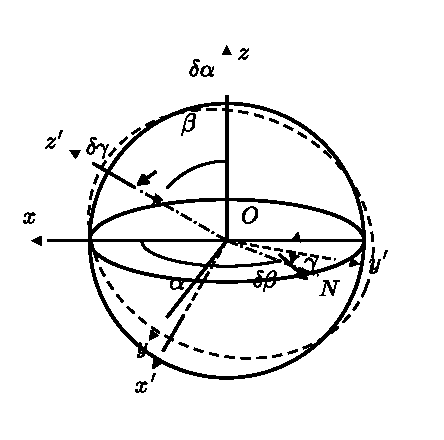
\includegraphics[width=6.5cm]{fig20.pdf}\\[0.3em]{\small 图 20}\end{minipage}\par\nopagebreak

与坐标轴的上述转动相应，整个变换矩阵等于(58.3)和(58.4)式的三个矩阵的乘积：
\begin{equation*}
  \hat{U}(\alpha,\beta,\gamma)=\hat{U}_z(\gamma)\hat{U}_y(\beta)\hat{U}_z(\alpha),
\end{equation*}
这些矩阵相乘后，我们最后得
\begin{equation}
  \hat{U}(\alpha,\beta,\gamma)=\left(\begin{array}{cc}
  \cos\dfrac{\beta}{2}\cdot e^{i(\alpha+\gamma)/2} &
  \sin\dfrac{\beta}{2}\cdot e^{-i(\alpha-\gamma)/2}\\[1.2em]
  -\sin\dfrac{\beta}{2}\cdot e^{i(\alpha-\gamma)/2} &
  \cos\dfrac{\beta}{2}\cdot e^{-i(\alpha+\gamma)/2}
  \end{array}\right).
\end{equation}
根据定义，高秩旋量可按一秩旋量的分量乘积进行变换.但是在物理应用中，我们感兴趣的不是旋量本身的变换规律，而是波函数 $\psi_{jm}$.

令函数组 $\psi_{jm}$（$m=j,j-1,\cdots,-j$）描述角动量具有定值 $j$ 的一个态，用的是 $xyz$ 坐标系，并令 $\psi_{jm}$ 描述同一个态但用 $x'y'z'$ 轴；前者的 $m$ 是 $j_z$ 的值，后者的 $m'$ 是 $j_{z'}$ 的值.这两组函数呈线性关系，我们把它写成下列形式：
\begin{equation}
  \psi_{jm}=\sum_{m'}D^{(j)}_{m'm}(\alpha,\beta,\gamma)\psi_{jm'}.
\end{equation}
系数 $D^{(j)}_{m'm}$ 对 $m'$ 和 $m$ 而言组成一个 $2j+1$ 维矩阵，称为有限转动矩阵 $\hat{D}^{(j)}$，它的矩阵元是 $x'y'z'$ 轴相对于 $xyz$ 轴转动的欧拉角 $\alpha,\beta,\gamma$ 的函数.

有限转动矩阵可以通过函数 $\psi_{jm}$ 的旋量表示构造出来.$j=\frac{1}{2}$ 时，两个函数 $\psi_{\frac{1}{2}m}$（$m=\pm\frac{1}{2}$）构成一秩协变旋量.按(56.13)，从 $x'y'z'$ 到 $xyz$ 的变换是由(58.6)式的矩阵 $\hat{U}$ 实现，故 $\hat{D}^{(1/2)}=\hat{U}$.\footnote{注意(58.7)中的矩阵指标，它相当于用 $\psi_{jm}$ 排成的行去乘矩阵 $\hat{D}^{(j)}$ 的列.(58.7)可写成 $\psi_{jm}=(\psi'_j\hat{D}^{(j)})_m$，与(56.13)式一致.}其矩阵元可写成
\begin{equation*}
  D^{(1/2)}_{m'm}=e^{im'\gamma}d^{(1/2)}_{m'm}(\beta)e^{im\alpha},
\end{equation*}
其中 $d^{(1/2)}_{m'm}(\beta)$ 的值见下表：
\begin{equation}
  d^{(1/2)}_{m'm}(\beta)=
  \begin{array}{c|cc}
  m'\!\diagdown\!m & \frac{1}{2} & -\frac{1}{2}\\ \hline
  \frac{1}{2} & \cos\frac{1}{2}\beta & \sin\frac{1}{2}\beta\\
  -\frac{1}{2} & -\sin\frac{1}{2}\beta & \cos\frac{1}{2}\beta
  \end{array}
\end{equation}
对任意的 $j$ 值，函数组 $\psi_{jm}$ 与 $2j$ 秩对称协变旋量分量的关系见(57.6)式.$2j$ 秩旋量分量的变换矩阵就是 $2j$ 个 $\hat{D}^{(1/2)}$ 矩阵的乘积，其中的每个矩阵作用在一个旋量指标上.把这个乘积乘出来，并写回到 $\psi_{jm}$，得到下列变换矩阵：
\begin{equation}
  D^{(j)}_{m'm}(\alpha,\beta,\gamma)
  =e^{im'\gamma}d^{(j)}_{m'm}(\beta)e^{im\alpha},
\end{equation}
函数 $d^{(j)}_{m'm}(\beta)$ 为\footnote{计算见 A.~R.~Edmonds, \textit{Angular Momentum in Quantum Mechanics} Princeton, 1957.(58.9)的 $D^{(j)}_{m'm}$ 定义和 Edmonds 书上采用的不同之处，在于对换了 $\alpha$ 和 $\gamma$.本书的定义在处理过程中显得更自然一些.}
\begin{equation}
\begin{aligned}
  d^{(j)}_{m'm}(\beta)={}&\left[\frac{(j+m')!\,(j-m')!}{(j+m)!\,(j-m)!}\right]^{1/2}
  \left(\cos\frac{\beta}{2}\right)^{m'+m}\times\\
  &\times\left(\sin\frac{\beta}{2}\right)^{m'-m}
  \mathrm{P}^{(m'-m,\ m'+m)}_{j-m'}(\cos\beta),
\end{aligned}
\end{equation}
其中
\begin{equation}
\begin{aligned}
  \mathrm{P}_n^{(a,b)}(\cos\beta)={}&\frac{(-1)^n}{2^n n!}
  (1-\cos\beta)^{-a}(1+\cos\beta)^{-b}\times\\
  &\times\left(\frac{\mathrm{d}}{\mathrm{d}\cos\beta}\right)^{\!n}
  \left[(1-\cos\beta)^{a+n}(1+\cos\beta)^{b+n}\right]
\end{aligned}
\end{equation}
称为雅可比多项式\footnote{关于这种多项式和超几何级数的关系.见数学附录§e 的(e.11)式.}.我们注意到
\begin{equation}
  \mathrm{P}_n^{(a,b)}(-\cos\beta)=(-1)^n\mathrm{P}_n^{(b,a)}(\cos\beta).
\end{equation}
函数 $d^{(j)}_{m'm}$ 具有一系列对称性质，这可从(58.11)和(58.12)式导出，但直接从转动变换系数的定义出发去求，比较简单.

矩阵 $\hat{D}^{(j)}$ 是么正的，它是转动变换矩阵，由于 $(\alpha,\beta,\gamma)$ 转动的逆变换是 $(-\gamma,-\beta,-\alpha)$，对实矩阵 $d^{(j)}$ 就有下列关系：
\begin{equation}
  d^{(j)}_{m'm}(-\beta)=d^{(j)}_{mm'}(\beta).
\end{equation}
下列各式也都成立：
\begin{equation}
  d^{(j)}_{m'm}(\beta)=d^{(j)}_{-m,-m'}(\beta),
\end{equation}
\begin{equation}
\left.\begin{aligned}
  d^{(j)}_{m'm}(\pi)&=(-1)^{j+m}\delta_{m',-m},\\
  d^{(j)}_{m'm}(-\pi)&=(-1)^{j-m}\delta_{m',-m},\\
  d^{(j)}_{m'm}(0)&=\delta_{m'm}.
\end{aligned}\right\}
\end{equation}
$j=\frac{1}{2}$ 时，由(58.8)式可知以上诸式显然成立；推广到任意的 $j$ 时，根据变换矩阵的上述构造方法，可知以上诸式成立.

转动 $\pi-\beta$ 角，可用 $\pi$ 角和 $-\beta$ 角两个相继转动来完成：
\begin{equation*}
\begin{aligned}
  d^{(j)}_{m'm}(\pi-\beta)
  &=\sum_{m''}d^{(j)}_{m'm''}(\pi)\,d^{(j)}_{m''m}(-\beta)=\\
  &=(-1)^{j-m'}d^{(j)}_{-m',m}(-\beta),
\end{aligned}
\end{equation*}
或利用(58.13)式可得
\begin{equation}
  d^{(j)}_{m'm}(\pi-\beta)=(-1)^{j-m'}d^{(j)}_{m,-m'}(\beta).
\end{equation}
绕同一轴转动两次，与转角的先后次序无关.先转 $-\beta$ 角再转 $\pi$ 角，将得同一结果.把此结果与(58.16)式比较，得到
\begin{equation}
  d^{(j)}_{m'm}(\beta)=(-1)^{m'-m}d^{(j)}_{-m',-m}(\beta).
\end{equation}
由(58.17)，(58.14)和(58.13)可得
\begin{equation}
  d^{(j)}_{m'm}(\beta)=(-1)^{m'-m}d^{(j)}_{mm'}(\beta)
  =(-1)^{m'-m}d^{(j)}_{m'm}(-\beta).
\end{equation}
应用(58.13)到(58.18)诸式，我们可以导出全矩阵元 $D^{(j)}_{m'm}$ 的各种对称性质.特别是，对复共轭函数有
\begin{equation}
  D^{(j)*}_{m'm}(\alpha,\beta,\gamma)=D^{(j)}_{m'm}(-\alpha,\beta,-\gamma)
  =(-1)^{m'-m}D^{(j)}_{-m',-m}(\alpha,\beta,\gamma).
\end{equation}
从数学上讲，矩阵 $\hat{D}^{(j)}$ 给出了旋转群的 $2j+1$ 维不可约么正表示（见后面§98）.因此有正交关系：
\begin{equation}
  \int D^{(j_1)*}_{m'_1m_1}(\alpha,\beta,\gamma)
  D^{(j_2)}_{m'_2m_2}(\alpha,\beta,\gamma)\,
  \frac{\mathrm{d}\omega}{8\pi^2}
  =\frac{1}{2j_1+1}\delta_{j_1j_2}\delta_{m_1m_2}\delta_{m'_1m'_2},
\end{equation}
其中 $\mathrm{d}\omega=\sin\beta\,\mathrm{d}\alpha\,\mathrm{d}\beta\,\mathrm{d}\gamma$.

函数组对下标 $m$ 和 $m'$ 的正交性为因子 $e^{i(m\alpha+m'\gamma)}$ 所保证；对指标 $j$ 的正交性来自 $d^{(j)}_{m'm}$，对此，有
\begin{equation}
  \int_0^{\pi}d^{(j_1)}_{m'm}(\beta)\,d^{(j_2)}_{m'm}(\beta)\cdot
  \frac{1}{2}\sin\beta\,\mathrm{d}\beta
  =\frac{1}{2j_1+1}\delta_{j_1j_2}.
\end{equation}
最后，为参考计，我们给出参量具有特殊值的几个 $d^{(j)}_{m'm}$ 函数的表式.对 $j=1$ 我们有
\begin{equation}
  d^{(1)}_{m'm}(\beta)=
  \begin{array}{c|ccc}
  m'\!\diagdown\!m & 1 & 0 & -1\\ \hline
  1 & \frac{1}{2}(1+\cos\beta) & \frac{1}{\sqrt{2}}\sin\beta & \frac{1}{2}(1-\cos\beta)\\[0.4em]
  0 & -\frac{1}{\sqrt{2}}\sin\beta & \cos\beta & \frac{1}{\sqrt{2}}\sin\beta\\[0.4em]
  -1 & \frac{1}{2}(1-\cos\beta) & -\frac{1}{\sqrt{2}}\sin\beta & \frac{1}{2}(1+\cos\beta)
  \end{array}
\end{equation}
对整数 $j=l$ 和 $m'=0$，由(58.10)和(58.11)式得
\begin{equation}
  d^{(l)}_{0m}(\beta)=(-1)^m d^{(l)}_{m0}(\beta)
  =(-1)^m\sqrt{\frac{(l-m)!}{(l+m)!}}\,\mathrm{P}_l^m(\cos\beta).
\end{equation}
此式的推导容易从原定义(58.7)式看出.我们把(58.7)右边的 $\psi_{jm'}$ 的值指定给 $z$ 轴，此轴上有（对 $j=l$）
\begin{equation}
  \mathrm{Y}_{lm'}(\boldsymbol{n}_{z'})=i^l\sqrt{\frac{2l+1}{4\pi}}\,\delta_{m'0}.
\end{equation}
式左的 $\psi_{jm}$ 就是球谐函数 $\mathrm{Y}_{lm}(\beta,\alpha)$，其球极角 $\varphi\equiv\alpha,\theta\equiv\beta$ 给出 $z'$ 轴的方向，将(58.24)代入(58.7)式，得
\begin{equation}
  \mathrm{Y}_{lm}(\beta,\alpha)=i^l\sqrt{\frac{2l+1}{4\pi}}\,
  D^{(l)}_{0m}(\alpha,\beta,\gamma),
\end{equation}
上式等同于(58.23)式.

最后，列出 $m$ 或 $m'$ 具有最大可能值时的函数表式：
\begin{equation}
\begin{aligned}
  d^{(j)}_{jm}(\beta)&=(-1)^{j-m}d^{(j)}_{mj}=\\
  &=\left[\frac{(2j)!}{(j+m)!\,(j-m)!}\right]^{1/2}
  \left(\cos\frac{\beta}{2}\right)^{j+m}
  \left(\sin\frac{\beta}{2}\right)^{j-m}
\end{aligned}
\end{equation}

\section{粒子的部分极化}

适当地选择 $z$ 轴的方向总能使所给旋量 $\psi^{\lambda}$（自旋为 $\frac{1}{2}$ 的粒子波函数）的一个分量（例如 $\psi^2$）等于零.这是因为空间方向由两个参量（两个角度）所确定，这就是说，可供我们使用的参量数，正好等于欲使一个分量为零（复分量 $\psi^2$ 的实部和虚部都等于零）的条件数.

从物理上讲来，这表明自旋为 $\frac{1}{2}$ 的粒子（为明确起见，我们把它说成是电子）如果处于某一自旋波函数所描述的态中，那就存在一个空间方向，该粒子沿此方向的自旋投影具有 $\sigma=\frac{1}{2}$ 的定值.处于这样的态中的电子可称为完全极化的.

但是也存在着另一种电子态，称为部分极化态.这种态是一个混合态（对自旋而言的混合态），不能用波函数描述，只能用密度矩阵加以描述（参考§14）.

电子的自旋密度矩阵或极化密度矩阵是一个二秩旋量 $\rho^{\lambda}_{\mu}$，满足以下归一化条件：
\begin{equation}
  \rho^{\lambda}_{\lambda}=\rho^1_1+\rho^2_2=1,
\end{equation}
并满足“厄米”条件：
\begin{equation}
  (\rho^{\lambda}_{\mu})^*=\rho^{\mu}_{\lambda}.
\end{equation}
在纯自旋态（即完全极化态）情形下，$\rho^{\lambda}_{\mu}$ 可以化成波函数 $\psi^{\lambda}$ 的分量乘积：
\begin{equation}
  \rho^{\lambda}_{\mu}=\psi^{\lambda}(\psi^{\mu})^*.
\end{equation}
密度矩阵的“对角”分量 $\rho^1_1$ 和 $\rho^2_2$ 确定了电子自旋的 $z$ 分量值为 $+\frac{1}{2}$ 和 $-\frac{1}{2}$ 的概率，因此该分量的平均值为
\begin{equation*}
  \bar{s}_z=\frac{1}{2}\left(\rho^1_1-\rho^2_2\right),
\end{equation*}
由(59.1)式得
\begin{equation}
  \rho^1_1=\frac{1}{2}+\bar{s}_z,\qquad
  \rho^2_2=\frac{1}{2}-\bar{s}_z.
\end{equation}
在纯态情形下，$s_\pm=s_x\pm is_y$ 的平均值由下式算出：
\begin{equation*}
\begin{aligned}
  \bar{s}_+&=\psi^{\lambda*}\hat{s}_+\psi^{\lambda}\\
  \bar{s}_-&=\psi^{\lambda*}\hat{s}_-\psi^{\lambda}
\end{aligned}
\end{equation*}
按(55.6)和(55.7)式，算符 $\hat{s}_{\pm}$ 由下列矩阵给出：
\begin{equation*}
  \hat{s}_+=\left(\begin{array}{cc}0&1\\0&0\end{array}\right),\qquad
  \hat{s}_-=\left(\begin{array}{cc}0&0\\1&0\end{array}\right),
\end{equation*}
我们得
\begin{equation*}
  \bar{s}_+=\psi^{1*}\psi^2,\qquad
  \bar{s}_-=\psi^{2*}\psi^1.
\end{equation*}
与此相应，在混合态中有
\begin{equation}
  \rho^1_2=\bar{s}_-,\qquad \rho^2_1=\bar{s}_+.
\end{equation}
采用泡利矩阵，可把(59.4)，(59.5)合并成
\begin{equation}
  \rho^{\lambda}_{\mu}=\frac{1}{2}
  \left(\delta^{\lambda}_{\mu}+2\hat{\sigma}^{\lambda}_{\mu}\cdot\bar{\boldsymbol{s}}\right).
\end{equation}
由此可见，电子极化密度矩阵的所有分量可以通过自旋矢量的分量平均值表出.换句话说，实矢量 $\bar{\boldsymbol{s}}$ 完全确定了自旋为 $\frac{1}{2}$ 的粒子的极化性质.在完全极化的情形下，这个矢量的一个分量（适当选择 $z$ 轴方向后）等于 $\frac{1}{2}$，另两个分量等于零.在非极化态的相反情形下，三个分量都等于零.在任意部分极化和任意坐标系的一般情形下，我们有不等式 $0\leqslant\rho\leqslant1$，其中的
\begin{equation*}
  \rho=2\left(\bar{s}_x^2+\bar{s}_y^2+\bar{s}_z^2\right)^{1/2},
\end{equation*}
称为电子的极化度.

自旋值为 $s$ 的粒子，密度矩阵是一个 $4s$ 秩旋量 $\rho^{\lambda\mu\cdots}{}_{\rho\sigma\cdots}$，对前 $2s$ 个指标和后 $2s$ 个指标都是对称的，并满足下列条件：
\begin{equation}
  \rho^{\lambda\mu\cdots}{}_{\lambda\mu\cdots}=1,
\end{equation}
\begin{equation}
  \left(\rho^{\lambda\mu\cdots}{}_{\rho\sigma\cdots}\right)^*
  =\rho^{\rho\sigma\cdots}{}_{\lambda\mu\cdots}.
\end{equation}
计算这个密度矩阵的独立分量数时，我们注意到指标 $\lambda,\mu,\cdots$（或 $\rho,\sigma,\cdots$）的各组可能值中，实际上只可能有 $2s+1$ 组不同的值，再考虑到 $\rho^{\lambda\mu\cdots}{}_{\rho\sigma\cdots}$ 诸分量间存在着(59.7)式的关系，因此不同分量数等于 $(2s+1)^2-1=4s(s+1)$.这些分量虽然都是复量，但(59.8)式表明并不因此而增加部分极化粒子态的独立分量数，它仍等于\footnote{给出了这些量等于同时给出了矢量 $\boldsymbol{s}$ 诸分量及其所有的 $2,3,\cdots,2s$ 次乘幂和乘积的诸平均值，这些量不能化成较低次的乘幂（参考§55 例题3）.} $4s(s+1)$.为比较起见，我们指出，粒子的完全极化态是由 $4s$ 个量确定的（$2s+1$ 个波函数的复分量 $\psi^{\lambda\mu\cdots}$，加上一个归一化条件和一个对描述状态而言并不重要的公共相因子）.

旋量 $\rho^{\lambda\mu\cdots}{}_{\rho\sigma\cdots}$ 和一切 $4s$ 秩旋量一样，等同于一组 $4s,4s-2,\cdots,0$ 秩不可约张量.在目前情形下，对每一个秩数讲来，只有一个不可约张量，这是由于旋量 $\rho^{\lambda\mu\cdots}{}_{\rho\sigma\cdots}$ 的对称性，每次缩并时只能有一种缩并方法：从 $\lambda,\mu,\cdots$ 中（任）选一个指标并从 $\rho,\sigma,\cdots$ 中选一个指标相缩并.除此以外，标量（0 秩张量）一般不存在，它由于条件(59.7)而变为 1.

\section{时间反演和克拉默定理}

量子力学中对时间变号所具的对称性，反映为下列事实，如果 $\psi$ 是该系统的某一定态波函数，则“时间反演”后的波函数（记作 $\psi^{\mathrm{T}}$）可以描述同一能量的某一可能态.在§18末曾经指出，$\psi^{\mathrm{T}}$ 等同于复共轭函数 $\psi^*$.这一简单结论，是对不考虑自旋的粒子波函数而言的.当有自旋时，尚需作进一步的修改.

我们把自旋为 $s$ 的粒子波函数写成逆变旋量 $\psi^{\lambda\mu\cdots}$（$2s$ 秩）形式.但当变成复共轭函数 $\psi^{\lambda\mu\cdots *}$ 后，这个函数却按协变旋量的分量变换.因此时间反演变换相当于把波函数 $\psi^{\lambda\mu\cdots}$ 变成这样一组新的波函数，它的协变分量按下式确定：
\begin{equation}
  \psi^{\mathrm{T}}_{\lambda\mu\cdots}=\psi^{\lambda\mu\cdots *}.
\end{equation}
给定了一组指标值 $\lambda,\mu,\cdots$ 后，一个旋量的协变分量和逆变分量，相当于不同符号的角动量投影值.因此用函数 $\psi_{s\sigma}$ 表示时，时间反演相当于把 $\psi_{s\sigma}$ 变成 $\psi_{s,-\sigma}$，这正是我们预料的结果，因为时间变号时要改变角动量的方向.由(60.1)式给出的精确关系为
\begin{equation}
  \psi^{\mathrm{T}}_{s,-\sigma}=\psi^*_{s\sigma}(-1)^{s-\sigma}.
\end{equation}
可见，时间反演操作所需的 $\psi_{s\sigma}\to\psi^*_{s\sigma}$ 变换意味着下列变换\footnote{注意球谐函数的复共轭规则，按(28.9)式，它与(60.3)的一般规则相一致.}：
\begin{equation*}
  \psi_{s\sigma}\longrightarrow\psi_{s,-\sigma}(-1)^{s-\sigma}.
\end{equation*}
重复操作一次后，得
\begin{equation}
  \psi_{s\sigma}\to\psi_{s,-\sigma}(-1)^{s-\sigma}
  \to\psi_{s\sigma}(-1)^{s-\sigma}(-1)^{s+\sigma}
  =\psi_{s\sigma}(-1)^{2s}.
\end{equation}
可见只有当自旋为整数时，两次时间反演使波函数回到原值：如果自旋为半整数，则波函数变号.

现在来研究任一多粒子系统，设粒子间具有相互作用.考虑了相对论性的相互作用以后，一般地说，这个系统的轨道角动量和自旋角动量不再分别守恒，只有总角动量 $\boldsymbol{J}$ 是守恒量.如果没有外场存在，该系统的每个能级具有 $2j+1$ 重简并，加入外场后简并有所解除.产生的问题是能否把简并完全解除，使该系统只有非简并能级.这个问题与时间反演对称性密切相关.

在经典电动力学中，如果时间变号时电场不变号而磁场变号，则方程具有不变性.\footnote{参考第二卷，《场论》§17.尚可参考后面§111 之末.}运动的这一基本性质，应该在量子力学中得到保持.因此，不但在封闭系统中，而且在任意外电场中（当磁场不存在时），都应具有时间反演对称性.

系统波函数是一些 $n$ 秩旋量 $\psi^{\lambda\mu\cdots}$，$n$ 两倍于所有粒子自旋之和$\left(n=2\sum s_a\right)$；这个和不一定等于该系统的总自旋 $S$.

如前所述，我们可以肯定，在任意电场中，波函数及其时间反演函数必须对应于具有相同能量的态.如果这个能级是非简并的，这两个态必须相同，即其波函数只能相差一个常因子［当然，两者都必须用同型的（协变或逆变的）旋量表出］.

令 $\psi^{\mathrm{T}}_{\lambda\mu\cdots}=C\psi_{\lambda\mu\cdots}$，或用(60.1)式写作
\begin{equation}
  \psi^{\lambda\mu\cdots *}=C\psi_{\lambda\mu\cdots},
\end{equation}
其中 $C$ 是一常数.上式两边都取复共轭，得
\begin{equation*}
  \psi^{\lambda\mu\cdots}=C^*\psi^*_{\lambda\mu\cdots}.
\end{equation*}
把式左的指标下降，同时把式右的指标上升.这相当于上式两边乘以 $g_{\alpha\lambda}g_{\beta\mu}\cdots$，并对 $\lambda,\mu,\cdots$ 等指标求和；同时在式右应用下列公式：
\begin{equation*}
  g_{\alpha\lambda}g_{\beta\mu}\cdots=(-1)^n g^{\lambda\alpha}g^{\mu\beta}\cdots.
\end{equation*}
结果得
\begin{equation*}
  \psi_{\lambda\mu\cdots}=C^*(-1)^n\psi^{\lambda\mu\cdots *}.
\end{equation*}
把(60.4)式的 $\psi^{\lambda\mu\cdots *}$ 代入上式，我们得
\begin{equation*}
  \psi_{\lambda\mu\cdots}=(-1)^n CC^*\psi_{\lambda\mu\cdots}.
\end{equation*}
此式应该恒等地得到满足，即必须有 $(-1)^n CC^*=1$.但由于 $|C|^2$ 永远是正的，显然，只有 $n$ 是偶数时（即和式 $\sum s_a$ 为整数时）才有可能.$n$ 为奇数时（$\sum s_a$ 为半整数时）条件(60.4)不能满足.\footnote{当和式 $\sum s_a$ 是整数（半整数）时，系统总自旋 $S$ 的所有可能值也都是整数（半整数）.}

由此得出结论，只有对粒子自旋之和为整数值的一个系统，电场才有可能完全解除简并.对于自旋之和为半整数的系统，在任意电场中所有的能级都必然是双重简并的\footnote{如果该电场具有高度的对称性（立方对称性），尚有可能存在四重简并（参考§99 及其习题）.}，两个复共轭旋量对应于具有同一能量的两个不同态\footnote{H.~A.~Kramers 1930.}.

再作一点数学方面的注释.具有实常数 $C$ 的(60.4)式，在数学上相当于旋量的诸分量能够对应于一组实量的条件，可以称作使旋量为“实”的条件\footnote{从字面上讲，把旋量称为实旋量的是没有意义的，因为它的复共轭旋量具有不同的变换规律.}.奇数的 $n$ 不能满足条件(60.4)，意味着没有一个实量能够对应于一个奇数秩的旋量.反之，对偶数的 $n$，条件(60.4)可以满足，$C$ 可以是实数.特别是，一个实矢量可以对应于一个二秩对称旋量，只要 $C=1$ 时(60.4)得到满足：
\begin{equation*}
  \psi^{\lambda\mu *}=\psi_{\lambda\mu}
\end{equation*}
［这不难从(57.8)和(57.9)看出］.$C=1$ 的(60.4)式实际上是任意偶数秩的对称旋量成为“实”量的条件.
